\section*{Ejercicios}\label{ejercicios}
\addcontentsline{toc}{section}{Ejercicios}

\begin{ejercicio}
¿Qué hace el siguiente programa? Haz una traza. 
\pythonexternal[frame=single]{code/ejercicio4_while1.py}
\end{ejercicio}

\begin{ejercicio}
¿Qué hace el siguiente programa? Haz una traza. 
\pythonexternal[frame=single]{code/ejercicio4_while2.py}
\end{ejercicio}

\begin{ejercicio}
¿Qué hace el siguiente programa? Haz una traza. 
\pythonexternal[frame=single]{code/ejercicio4_while3.py}
\end{ejercicio}

\begin{ejercicio}
¿Qué hace el siguiente programa? Haz una traza. 
\pythonexternal[frame=single]{code/ejercicio4_while4.py}
\end{ejercicio}

\begin{ejercicio}

Escribe un programa que lea repetidamente números
hasta que el usuario introduzca ``fin''. Una vez se haya introducido
``fin'', muestra por pantalla el total, la cantidad de números y la
media de esos números. Si el usuario introduce cualquier otra cosa que
no sea un número, detecta su fallo usando \pythoninline{try} y
\pythoninline{except}, muestra un mensaje de error y pasa al número
siguiente.

La ejecución del programa debe dar lugar a lo siguiente:\\

\begin{Verbatim}[frame=single, label={\em ejemplo de ejecución}]
>>> %Run
  Introduzca un número: 4
  Introduzca un número: 5
  Introduzca un número: dato erróneo
  Entrada inválida
  Introduzca un número: 7
  Introduzca un número: fin
  16 3 5.33333333333
\end{Verbatim}

Ejecute pruebas a través de la consola y verifique la salida. ¿Tu programa funciona con números negativos? ¿Funciona con números reales? 
\end{ejercicio}


\begin{ejercicio}
 Implementar un programa que lea 5 números enteros y positivos y calcule la media de los números y lo presenta con máximo 1 decimal. Cuando el usuario mete un numero negativo o otra entrada inválida, hay que volver a preguntárselo. La lectura de los números tienes que hacer dentro de un bucle (entonces no simplemente llamar 5 veces a input en secuencia!). 
 
Ejecuta los siguientes test cases para testear tu programa:\\

\begin{Verbatim}[frame=single, label={\em ejemplo de ejecución}]
>>> %Run 
Introduzca un número: 3
Introduzca un número: 4
Introduzca un número: 0
Introduzca un número: 2
Introduzca un número: 10
La media de los 5 numeros es 19/5 = 3.8
>>> %Run 
Introduzca un número: -2
Solo numeros positivos!
Introduzca un número: 2
Introduzca un número: 4
Introduzca un número: r
Entrada inválida
Introduzca un número: 7
Introduzca un número: 10
Introduzca un número: 0
La media de los 5 numeros es 23/5 = 4.6
\end{Verbatim}

\end{ejercicio}

\begin{ejercicio} 
Escribe un programa que recibe un número entero $M$, genere todos los números múltiplos de 3 que hay entre 1 y $M$. Ejecuta los siguientes test cases para testear tu programa:\\

\begin{Verbatim}[frame=single, label={\em ejemplo de ejecución}]
>>> %Run 
Introduzca un número: 2
No hay multiplos de 3.
>>> %Run 
Introduzca un número: 3
3
>>> %Run 
Introduzca un número: -1
No hay multiplos de 3.
>>> %Run 
Introduzca un número: -8
-3,-6
>>> %Run 
Introduzca un número: 30
3,6,9,12,15,18,21,24,27,30
>>> %Run 
Introduzca un número: r
Entrada inválida
Introduzca un número: hi
Entrada inválida
Introduzca un número: 10
3,6,9
\end{Verbatim}
\end{ejercicio}


\begin{ejercicio}
¿Qué hace el siguiente programa? Haz trazas.

\pythonexternal[frame=single]{code/ejercicio_for.py}

¿Cuál será el resultado del programa si los datos introducidos son 3 y 6? ¿Por qué?
¿Y si los datos introducidos fuesen 7 y 7?
¿El resultado del programa depende del orden en que son introducidos los datos? ¿Por qué?
Expresar con una fórmula qué cálculo hace este programa cuando a <= b.

\end{ejercicio}


\begin{ejercicio}
¿Qué hace el siguiente programa? Haz trazas.

\pythonexternal[frame=single]{code/ejercicio_for1.py}
\end{ejercicio}

\begin{ejercicio}
¿Qué hace el siguiente programa? Haz trazas.

\pythonexternal[frame=single]{code/ejercicio_for2.py}
\end{ejercicio}

\begin{ejercicio}
¿Qué hace el siguiente programa? Haz trazas.

\pythonexternal[frame=single]{code/ejercicio_for3.py}
\end{ejercicio}



\begin{ejercicio} 
Modificar el programa anterior para que visualice sólo aquellos múltiplos de 3 entre 1 y $M$ que no son divisibles entre 2. Ejecuta los siguientes test cases para testear tu programa:

\begin{tabular}{|l|l|l|l|}
\hline
test case ID  & inputs & expected outputs  \\ 
\hline\hline
1 & 0 & no hay múltiplos de 3\\
2 & 2 & no hay múltiplos de 3\\
3 & -1 & no hay múltiplos de 3\\
4 & -22 & -3,-9,-15,-21\\
5 & 21 & 3,9,15,21\\
6 & 66 & 3,9,15,21,27,33,39,45,51,57,63\\
\hline
\end{tabular}
\end{ejercicio}


\begin{ejercicio}
Escribe un programa que imprime la tabla de multiplicar, como la tabla pitagórica (denominada así en honor de Pitagoras (\url{https://es.wikipedia.org/wiki/Pitagoras})). La primera fila y la primera columna contienen los números que se van a multiplicar (habitualmente, los números de 1 hasta el 10), y en la intersección de cada fila y cada columna está el producto del número de su fila por el número de su columna.


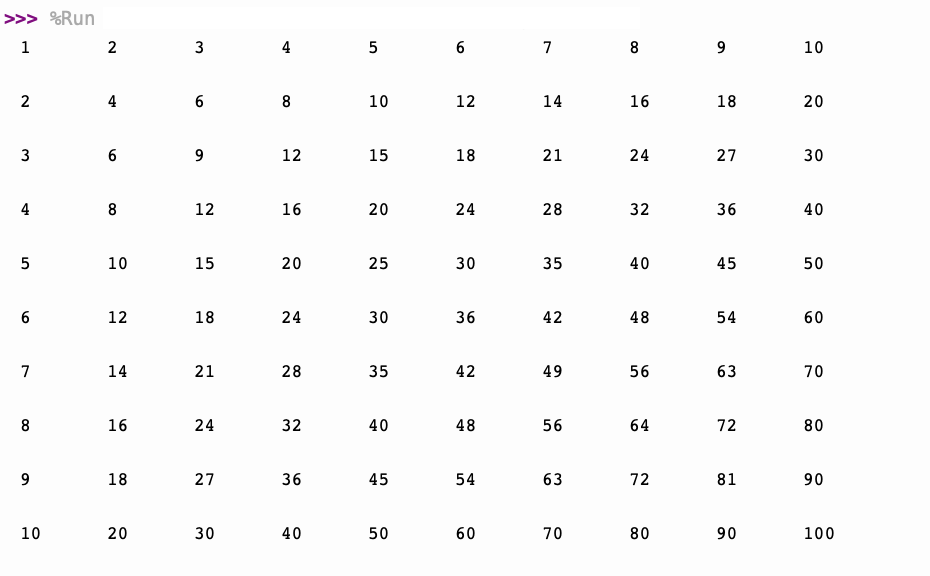
\includegraphics[width=0.75\textwidth]{images/pitagoras.png}
  

\end{ejercicio}

\newpage

\begin{ejercicio}
Escribir un programa en Python para imprimir los valores ASCII de todos los caracteres que hemos visto usando for loop. Por ejemplo, hemos visto lo en Figura \ref{ascii}.

\begin{figure}
    \centering
    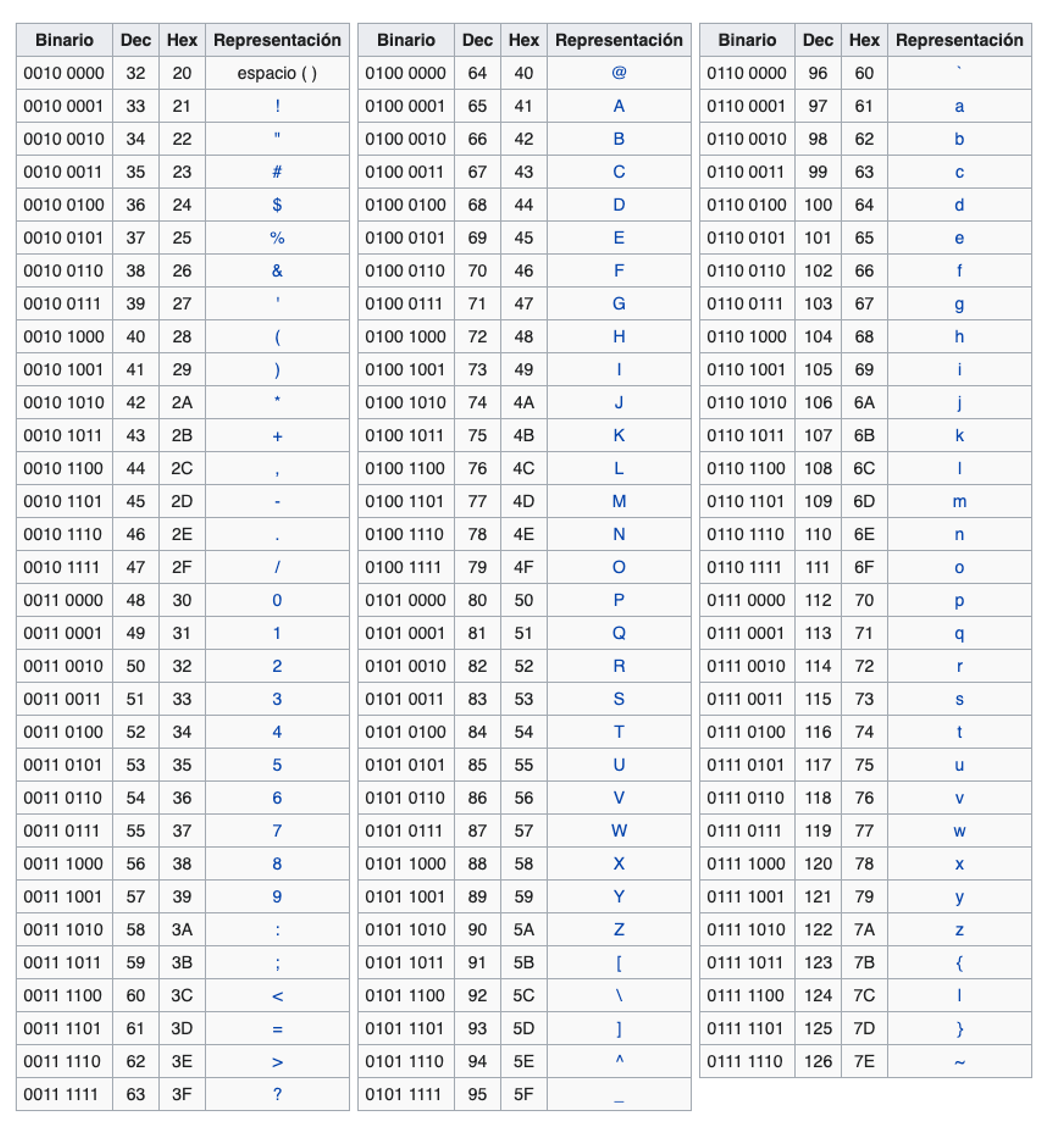
\includegraphics[width=0.8\textwidth]{book/Spanish/03_Conditionals_if_elif_else/images/ASCII.png}
    \caption{ASCII código}
    \label{ascii}
\end{figure}

\begin{small}
\begin{Verbatim}[frame=single, label={\em ejemplo de ejecución}]
>>> %Run 
character   tiene codigo 32
character ! tiene codigo 33
character " tiene codigo 34
character # tiene codigo 35
character $ tiene codigo 36

.....

character | tiene codigo 124
character } tiene codigo 125
character ~ tiene codigo 126
>>> 
\end{Verbatim}
\end{small}
\end{ejercicio}

\begin{ejercicio}
Un número fuerte es un número especial cuya suma de factorial de dígitos es igual al número original.
Por ejemplo: 145 es un número fuerte. Desde, 1! + 4! + 5! = 145

Escriba un programa para ingresar el número del usuario y verifique si el número es un número fuerte o no.
\end{ejercicio}


\begin{ejercicio}
Escribe un programa que pide una palabra al usuario y lo imprime en un triangulo. Por ejemplo así:\\

\begin{small}
\begin{verbatim}
>>> %Run 
Give me a word: python
p
py
pyt
pyth
pytho
python
>>> %Run 
Give me a word: programacion
p
pr
pro
prog
progr
progra
program
programa
programac
programaci
programacio
programacion
>>> 
\end{verbatim}
\end{small}
\end{ejercicio}

\begin{ejercicio}
En 1914, el matemático indio Ramanujan descubrió la fórmula para calcular Pi que converge rápidamente. En 1987, los hermanos Chudnovsky descubrieron la fórmula de tipo Ramanujan que converge más rápidamente. Da lugar a tres formulas 

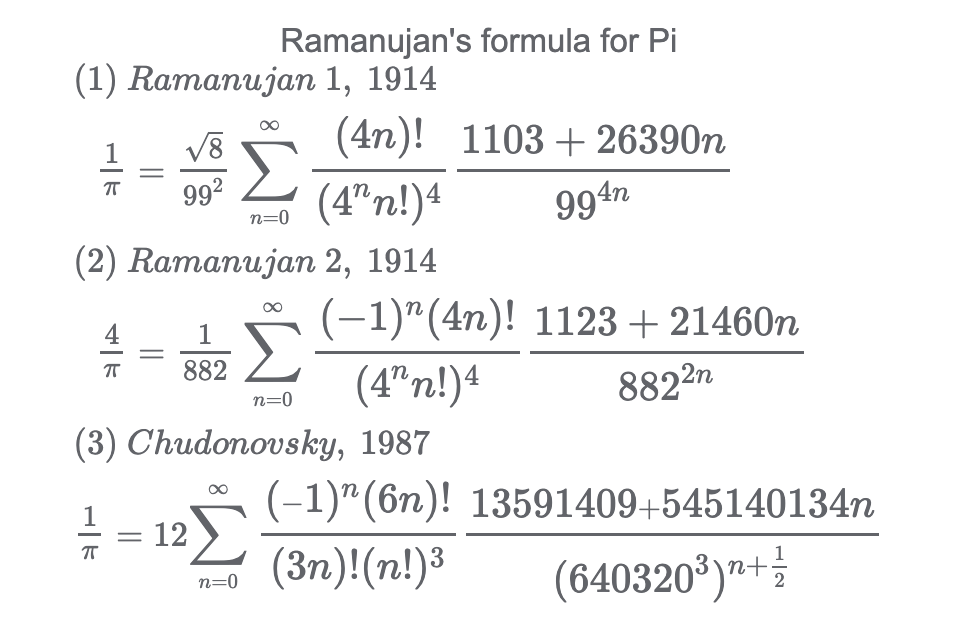
\includegraphics[width=10cm]{book/Spanish/04_Bucles/images/pi_aproxis.png}

Implementa las tres aproximaciones y, para hacer testing de tu implementación, compararlo con pi:

\begin{python}
import math

approximation_ramanujan1 =  
approximation_ramanujan2 =  
approximation_chudonovsky =  

print("Testing the solution")
print("Approximation Ramanujan 1 of pi:", approximation_ramanujan1)
print("Approximation Ramanujan 2 of pi:", approximation_ramanujan2)
print("Approximation Chudonovsky of pi:", approximation_chudonovsky)
print("Actual value of pi:", math.pi)    
\end{python}


\end{ejercicio}

